\documentclass[11pt, oneside]{article}   	% use "amsart" instead of "article" for AMSLaTeX format
\usepackage{geometry}                		% See geometry.pdf to learn the layout options. There are lots.
\geometry{letterpaper}                   		% ... or a4paper or a5paper or ... 
%\geometry{landscape}                		% Activate for for rotated page geometry
%\usepackage[parfill]{parskip}    		% Activate to begin paragraphs with an empty line rather than an indent
\usepackage{graphicx}				% Use pdf, png, jpg, or eps� with pdflatex; use eps in DVI mode
								% TeX will automatically convert eps --> pdf in pdflatex		
\usepackage{amssymb}
\usepackage{amsmath}
\usepackage{parskip}
\usepackage{color}
\usepackage{hyperref}

\title{scratch}
%\author{The Author}
%\section{}
%\subsection*{}
\date{}							% Activate to display a given date or no date

\graphicspath{{/Users/telliott_admin/Dropbox/Tex/png/}}
% \begin{center} 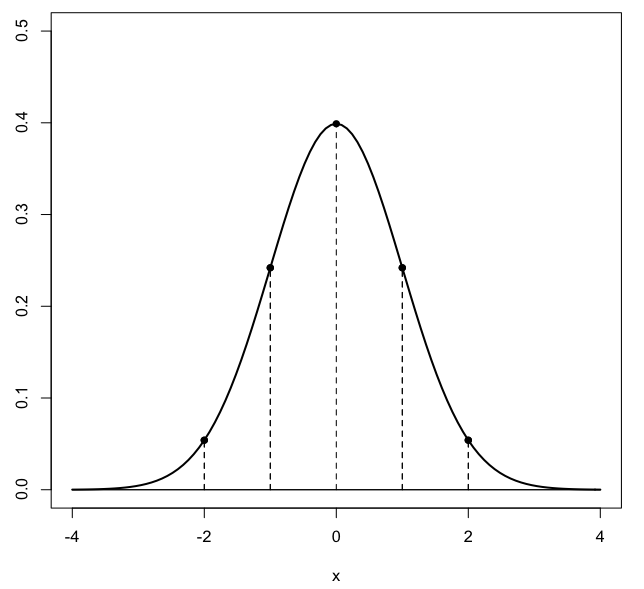
\includegraphics [scale=0.4] {gauss3.png} \end{center}
\begin{document}
\maketitle
\Large
Consider a cone with its vertex at the origin, opening up.  The equation is
\[ z = a \sqrt{x^2 + y^2} \]
where $a$ is a constant.

We can see that this is correct by considering what happens in the $xz$-plane when $y=0$.  Then $z = ax$ is a straight line with slope $a$.  Similarly, in the $yz$-plane we obtain $z = ay$.  Also, the level curves of $z$ are
\[ z = c = a \sqrt{x^2 + y^2} \]
where $c$ is  some other constant.  So
\[ c^2 = a^2(x^2 + y^2) = a^2r^2 \]
The level curves are seen to be circles with radius
\[ r = \frac{c}{a} \]
\subsection*{volume}
Now, we are asked to compute the volume under the graph of $z$ over the region of the unit disk.

We can set up the double integral as
\[ V = \int_{x = -1}^{x = 1} \int_{y = -\sqrt{1-x^2}}^{y = \sqrt{1-x^2}} a \sqrt{x^2 + y^2} \ dx \ dy \]
We can (and will) do this integral but it looks hard!  

In any problem with radial symmetry, you should probably try to switch to coordinates with the same symmetry.  Here, we switch to cylindrical coordinates (polar for $x$ and $y$, plus $z$).

The radius of the region $r$ is equal to 
\[ z = a \sqrt{x^2 + y^2} \]
so the volume is
\[ V = \int_{\theta = 0}^{\theta = 2 \pi} \int_{r=0}^{r=1} ar \ dA \]
where the area element is:
\[ dA = r \ dr \ d \theta \]
so
\[ V = \int_{\theta = 0}^{\theta = 2 \pi} \int_{r=0}^{r=1} ar \ r \ dr \ d \theta \]
The inner integral is
\[ a \int_0^1 r^2 \ dr = \frac{r^3}{3} \ \bigg |_0^1 = \frac{a}{3} \]
The outer integral is 
\[ \frac{a}{3} \ \int_0^{2\pi} d \theta = \frac{2}{3} \pi a \]

In this problem, we integrated over the unit disk, so the base of the cylindrical region and the inverted cone is just $1$.  The height is $z = a$.  From standard geometry, the cylinder enclosing the whole region has volume $\pi a$.  The cone has volume $1/3$ of that, so the volume we seek is the difference, which is $2/3 \pi a$ as we calculated.

I promised we would do this integral:
\[ V = \int_{x = -1}^{x = 1} \int_{y = -\sqrt{1-x^2}}^{y = \sqrt{1-x^2}} a \sqrt{x^2 + y^2} \ dx \ dy \]
Let's do the first quadrant and multiply by $4$.
\[ V = \int_{0}^{1} \int_{0}^{\sqrt{1-x^2}} a \sqrt{x^2 + y^2} \ dx \ dy \]
Remember the factor of $a$ (and the factor of $4$) for later.  

The inner integral is
\[ \int \sqrt{x^2 + y^2} \ dx \]
(with $x$ a constant).  So as not to be confused, replace $x$ by $c$ for now:
\[ \int \sqrt{c^2 + y^2} \ dy \]
We could remove the $c$ by scaling and then we will have something like $\sqrt{1 + y^2}$ which will still require a trig substitution.  So let's just move forward without that step.  Let
\[ \frac{y}{c} = \tan t \]
\[ y = c \tan t \]
\[ dy = c \sec^2 t \]
\[ \sqrt{c^2 + y^2}= c \sec t \]
So the integral is
\[ c^2 \int sec^3 t \ dt \]
We did solve this way back when, but I am just going to look it up in a table of integrals:
\[ = \int \sec^3 t \ dt = \frac{1}{2} \sec t \tan t + \frac{1}{2} \ln |\sec t + \tan t| + C \]
What are the bounds on $t$?  We had $y = 0 \rightarrow \sqrt{c^2 + y^2}$ and so $t = 0 \rightarrow \pi/2$.

At the upper bound we have
\[ 



\end{document}  